% Best one-variable GPY ratio against k (generated by a script).
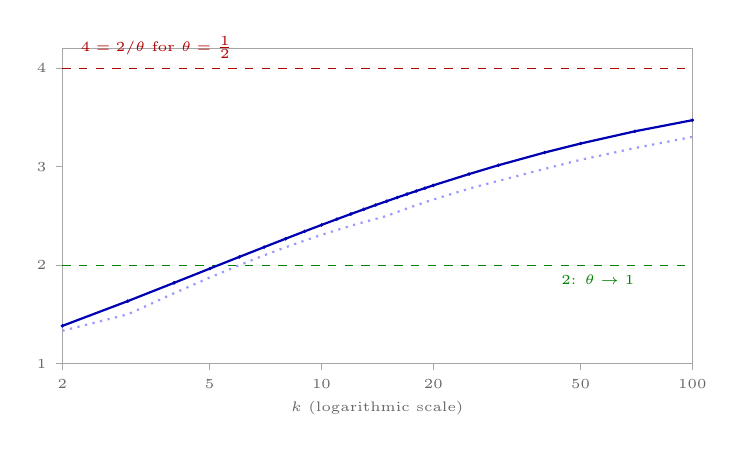
\begin{tikzpicture}[x=1cm,y=1cm]
\draw[black!35] (0,0) rectangle (8.00,4.00);
\draw[black!35] (0,0.00)--(-0.08,0.00) node[left,font=\tiny,black!60]{$1$};
\draw[black!35] (0,1.25)--(-0.08,1.25) node[left,font=\tiny,black!60]{$2$};
\draw[black!35] (0,2.50)--(-0.08,2.50) node[left,font=\tiny,black!60]{$3$};
\draw[black!35] (0,3.75)--(-0.08,3.75) node[left,font=\tiny,black!60]{$4$};
\draw[black!35] (0.00,0)--(0.00,-0.08) node[below,font=\tiny,black!60]{$2$};
\draw[black!35] (1.87,0)--(1.87,-0.08) node[below,font=\tiny,black!60]{$5$};
\draw[black!35] (3.29,0)--(3.29,-0.08) node[below,font=\tiny,black!60]{$10$};
\draw[black!35] (4.71,0)--(4.71,-0.08) node[below,font=\tiny,black!60]{$20$};
\draw[black!35] (6.58,0)--(6.58,-0.08) node[below,font=\tiny,black!60]{$50$};
\draw[black!35] (8.00,0)--(8.00,-0.08) node[below,font=\tiny,black!60]{$100$};
\node[below,font=\tiny,black!60] at (4.00,-0.35) {$k$ (logarithmic scale)};
\draw[red!70!black,dashed] (0,3.75)--(8.00,3.75) node[pos=0.15,above,font=\tiny]{$4=2/\theta$ for $\theta=\frac12$};
\draw[green!50!black,dashed] (0,1.25)--(8.00,1.25) node[pos=0.85,below,font=\tiny]{$2$: $\theta\to1$};
\draw[blue!70!black,thick] (0.000,0.479) -- (0.829,0.793) -- (1.417,1.025) -- (1.874,1.207) -- (2.247,1.355) -- (2.562,1.479) -- (2.835,1.586) -- (3.076,1.679) -- (3.291,1.761) -- (3.486,1.834) -- (3.664,1.900) -- (3.828,1.959) -- (3.979,2.014) -- (4.120,2.063) -- (4.252,2.109) -- (4.376,2.152) -- (4.493,2.191) -- (4.604,2.228) -- (4.709,2.263) -- (5.165,2.407) -- (5.538,2.519) -- (6.126,2.681) -- (6.583,2.795) -- (7.271,2.950) -- (8.000,3.091);
\draw[blue!40,thick,dotted] (0.000,0.417) -- (0.829,0.625) -- (1.417,0.893) -- (1.874,1.094) -- (2.247,1.250) -- (2.562,1.375) -- (2.835,1.477) -- (3.076,1.562) -- (3.291,1.635) -- (3.486,1.696) -- (3.664,1.750) -- (3.828,1.797) -- (3.979,1.838) -- (4.120,1.875) -- (4.252,1.925) -- (4.376,1.970) -- (4.493,2.011) -- (4.604,2.049) -- (4.709,2.083) -- (5.165,2.222) -- (5.538,2.321) -- (6.126,2.473) -- (6.583,2.588) -- (7.271,2.737) -- (8.000,2.879);
\fill[blue!70!black] (0.000,0.479) circle (0.7pt);
\fill[blue!70!black] (0.829,0.793) circle (0.7pt);
\fill[blue!70!black] (1.417,1.025) circle (0.7pt);
\fill[blue!70!black] (1.874,1.207) circle (0.7pt);
\fill[blue!70!black] (2.247,1.355) circle (0.7pt);
\fill[blue!70!black] (2.562,1.479) circle (0.7pt);
\fill[blue!70!black] (2.835,1.586) circle (0.7pt);
\fill[blue!70!black] (3.076,1.679) circle (0.7pt);
\fill[blue!70!black] (3.291,1.761) circle (0.7pt);
\fill[blue!70!black] (3.486,1.834) circle (0.7pt);
\fill[blue!70!black] (3.664,1.900) circle (0.7pt);
\fill[blue!70!black] (3.828,1.959) circle (0.7pt);
\fill[blue!70!black] (3.979,2.014) circle (0.7pt);
\fill[blue!70!black] (4.120,2.063) circle (0.7pt);
\fill[blue!70!black] (4.252,2.109) circle (0.7pt);
\fill[blue!70!black] (4.376,2.152) circle (0.7pt);
\fill[blue!70!black] (4.493,2.191) circle (0.7pt);
\fill[blue!70!black] (4.604,2.228) circle (0.7pt);
\fill[blue!70!black] (4.709,2.263) circle (0.7pt);
\fill[blue!70!black] (5.165,2.407) circle (0.7pt);
\fill[blue!70!black] (5.538,2.519) circle (0.7pt);
\fill[blue!70!black] (6.126,2.681) circle (0.7pt);
\fill[blue!70!black] (6.583,2.795) circle (0.7pt);
\fill[blue!70!black] (7.271,2.950) circle (0.7pt);
\fill[blue!70!black] (8.000,3.091) circle (0.7pt);
\end{tikzpicture}
